%
% Berechnung von Stromverteilungen mit Hilfe der Kirchhoffschen Regeln,
% Anwendung fuer Kapitel 1, beinhaltet auch das Nerd Sniping Problem
%
\index{Kirchhoff!Gustav Robert}
\index{Kirchhoff!Regeln}
\index{Kirchhoff!Gesetze|see{Kirchoff!Regeln}}
\index{Widerstandsnetzwerk}
Gustav Robert Kirchhoff hat in einer Arbeit 1847 gezeigt, wie sich
die Spannungen und Str"ome in einem Widerstandsnetzwerk berechnen
lassen. Dazu hat er zwei Regeln aufgestellt, mit deren Hilfe
sich ein lineares Gleichungssystem zur Berechnung der Spannungen
und Str"ome aufstellen l"asst.
\index{Stroemung@Str\"omung}
\index{Rohr}
\index{laminar}
\index{turbulent}
Seine Gesetze sind allerdings
nicht nur auf elektrische Str"ome anwendbar, sondern auch auf
Fl"ussigkeitsstr"ome durch ein Rohrnetz, solange die
Str"omungsgeschwindigkeiten so klein sind, dass die Str"omung als
laminar (nicht turbulent) betrachtet werden kann.

\subsection{Die Kirchhoffschen Gesetze\label{appkirchhoff}}
Kirchhoff ging aus von einem Netzwerk von ``Dr"ahten'' mit gegebenen
Widerstand und ``elektromotorischen Kr"aften'', die in diesen
Dr"ahten stecken. Ein Netzwerk dieser Art zeigt
Abbildung~\ref{kirchhoff-netzwerk}.
\begin{figure}
\begin{center}
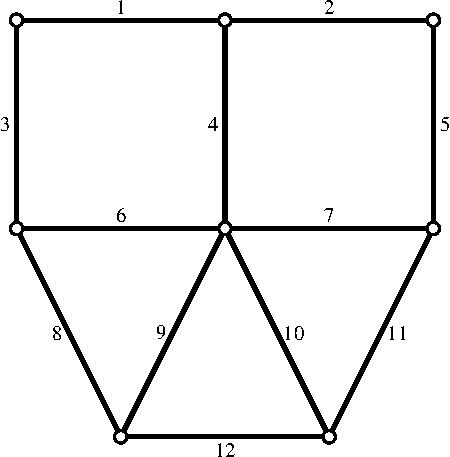
\includegraphics[width=0.6\hsize]{images/kirchhoff-1}
\end{center}
\caption{Netzwerk von Dr"ahten nach Kirchhoff\label{kirchhoff-netzwerk}}
\end{figure}
\index{Draht}
\index{Strom}
\index{elektromotorische Kraft}

\subsubsection{Das erste Gesetz: die Maschenregel}
In der zitierten Arbeit wird das erste Gesetz wie folgt formuliert:
\bigskip
\begin{center}
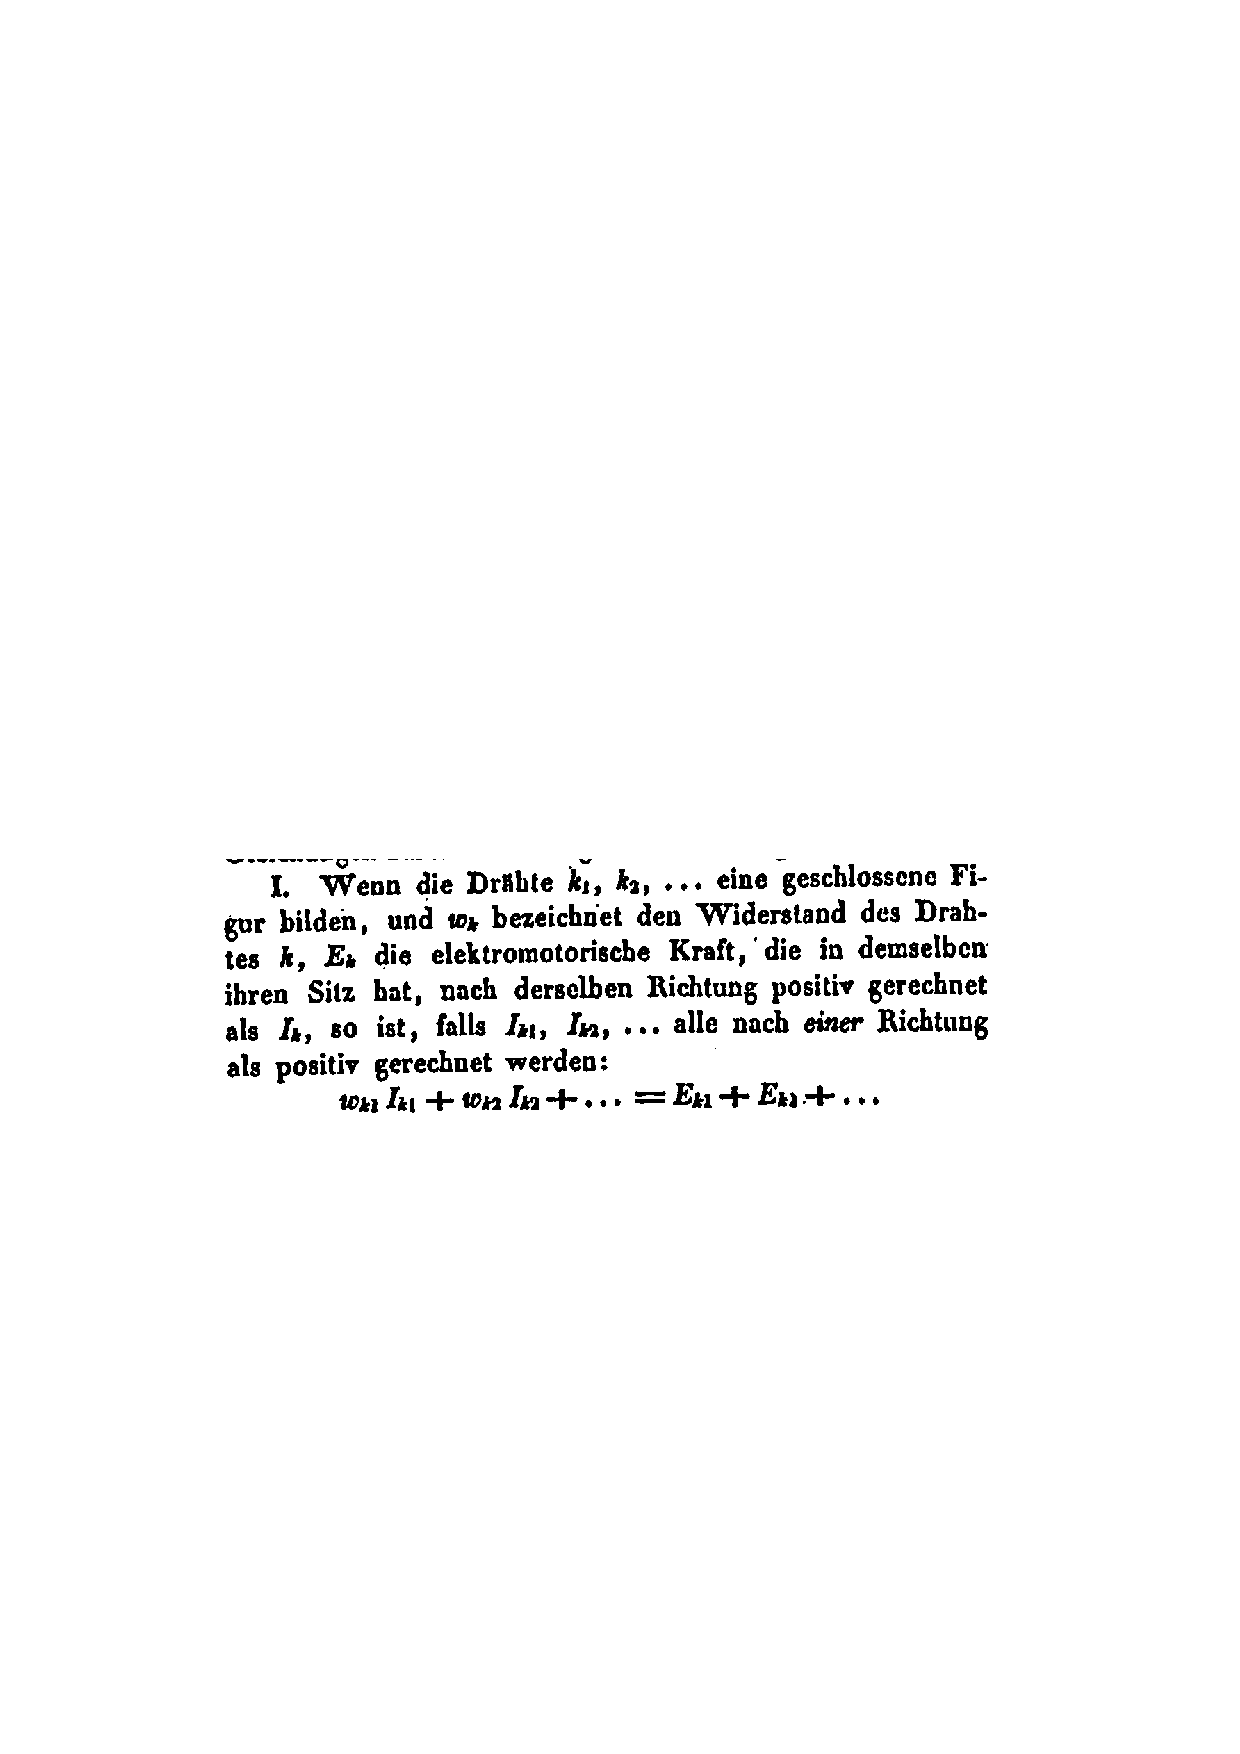
\includegraphics[width=\hsize]{graphics/kh1}
\end{center}
\bigskip
In unserer moderneren Schreibweise bezeichnen wir den Widerstand des
Drahtes mit der Nummer $k$ mit $R_k$. Da wir ausserdem nur an der
Mathematik interessiert sind, machen wir uns "uber die Interpretation
der ``elektromotorischen Kr"afte'' $E_k$ keine Gedanken. Die Gleichung,
die zu einer ``geschlossenen Figur'' geh"ort, ist also
\[
R_{k_1}I_{k_1}+
R_{k_2}I_{k_2}+
\dots + R_{k_s}I_{k_s}=
E_{k_1}+E_{k_2}+\dots+E_{k_s}.
\]
Doch was genau ist eine ``geschlossene Figur''? Der Begriff wird
in dem Aufsatz von Kirchhoff nicht definiert.
\index{Maschenregel}
\index{1. Kirchhoffsches Gesetz|see{Maschenregel}}

\subsubsection{Zyklen}
Zun"achst besteht eine ``geschlossene Figur'' immer aus einzelnen
Kanten des Netzwerks. Weiss man, welche Kanten dazu geh"oren, kann
man auch sofort ableiten, in welcher Reihenfolge sie vom Strom
durchflossen werden. Wirklich wichtig ist dies zwar auch nicht,
Kirchhoff sagt ja, es kommt nur auf die Summe an. Eine 
Figur ist also nur die Information, wie oft eine Kante des Netzwerkes darin
vorkommt. Wir k"onnen einer Figur also einen Vektor $f$ mit ganzen
Zahlen $f_i$ zuordnen, die angeben, wie oft die Kante $i$ in der
Figur vorkommt.
\begin{figure}
\begin{center}
\begin{tabular}{ccc}
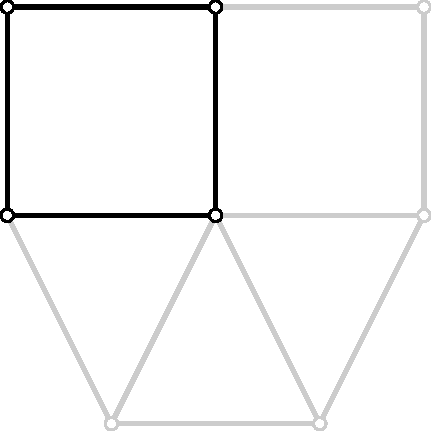
\includegraphics[width=0.25\hsize]{images/kirchhoff-3}&
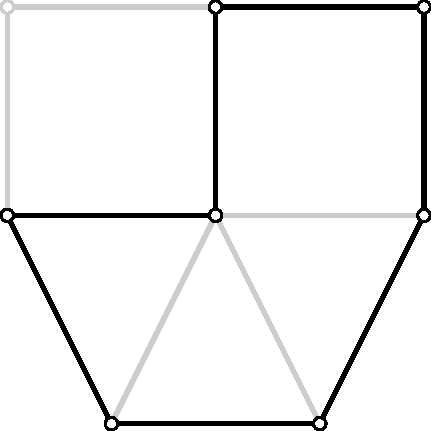
\includegraphics[width=0.25\hsize]{images/kirchhoff-4}&
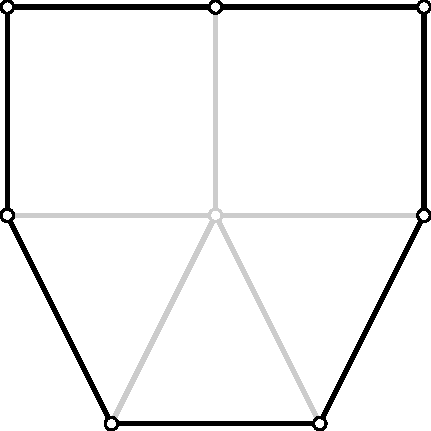
\includegraphics[width=0.25\hsize]{images/kirchhoff-5}
\\
$f_1$&$f_2$&$f_3$
\end{tabular}
\end{center}
\caption{Drei verschiedene Zyklen in dem Netzwerk von Abbildung~\ref{kirchhoff-netzwerk}
\label{kirchhoff-zyklen}}
\end{figure}

\index{Zyklus}
Eine geschlossene Figur zeichnet sich dadurch aus, dass es zu
jeder Kante eine n"achste Kante gibt, in der der Strom weiterfliessen
kann. In den Knoten des Netzwerkes kommen die Kanten zusammen,
zu jeder Kante, die im Knoten $j$ endet, braucht es eine zweite
Kante, die dort beginnt.
Es spielt jetzt also eine Rolle, in welcher Richtung eine
Kante durchlaufen wird, dies kann durch die Vorzeichen der $f_i$
ausgedr"uckt werden. Ausserdem w"ahlen wir f"ur jede Kante
des Netzwerkes eine Orientierung, zum Beispiel diejenige vom
Knoten mit der kleineren Nummer zu dem mit der gr"osseren,
und teilen dem Anfangspunkt
das Gewicht $-1$ und dem Endpunkt das Gewicht $+1$ zu. Die
aufaddierten Gewichte der Endpunkte einer Figur m"ussen in jedem
Knoten $0$ ergeben, damit die Figur geschlossen ist.
\begin{figure}
\begin{center}
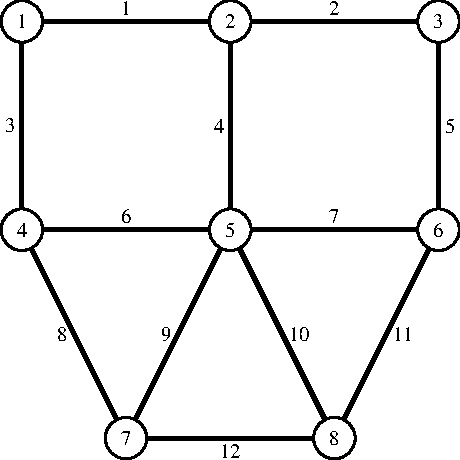
\includegraphics[width=0.6\hsize]{images/kirchhoff-2}
\end{center}
\caption{Numerierte Knoten im Netzwerk\label{netzwerk-numeriert}}
\end{figure}
Auch die Gewichte auf den einzelnen Knoten kann man mit einem
Vektor darstellen. Zu jeder Kante gibt es jetzt also einen
Vektor von Gewichten, die zusammen in eine Matrix $\partial$
geschrieben werden k"onnen.
F"ur das Beispielnetzwerk aus Abbildung~\ref{netzwerk-numeriert}
findet man f"ur diese Matrix
\setcounter{MaxMatrixCols}{12}
\[
\partial=\begin{pmatrix}
-1& 0&-1& 0& 0& 0& 0& 0& 0& 0& 0& 0\\
 1&-1& 0&-1& 0& 0& 0& 0& 0& 0& 0& 0\\
 0& 1& 0& 0&-1& 0& 0& 0& 0& 0& 0& 0\\
 0& 0& 1& 0& 0&-1& 0&-1& 0& 0& 0& 0\\
 0& 0& 0& 1& 0& 1&-1& 0&-1&-1& 0& 0\\
 0& 0& 0& 0& 1& 0& 1& 0& 0& 0&-1& 0\\
 0& 0& 0& 0& 0& 0& 0& 1& 1& 0& 0&-1\\
 0& 0& 0& 0& 0& 0& 0& 0& 0& 1& 1& 1
\end{pmatrix}
\]
Die Zeilen dieser Matrix sind numeriert mit den Knotennummern,
die Spalten mit den Kantennummern des Netzwerks. $\partial$
heisst auch der Randoperator des Netzwerks.
\index{Randoperator}

F"ur einen Vektor $f$, der eine Figur beschreibt, berechnet diese
Matrix die aufsummierten Gewichte in jedem Knoten.
Zu den drei Figuren in Abbildung~\ref{kirchhoff-zyklen} geh"oren
die folgenden drei Vektoren, die Wirkung der Matrix $\partial$
macht diese alle zum Nullvektor:
\[
f_1=\begin{pmatrix}
1\\0\\-1\\1\\0\\-1\\0\\0\\0\\0\\0\\0
\end{pmatrix},
%\quad
%\partial f_1
%=0%\begin{pmatrix}0\\0\\0\\0\\0\\0\\0\\0\end{pmatrix},
%,
\qquad
f_2=\begin{pmatrix}
0\\1\\0\\-1\\1\\1\\0\\-1\\0\\0\\1\\-1
\end{pmatrix},
%\quad
%\partial f_2
%=0%\begin{pmatrix}0\\0\\0\\0\\0\\0\\0\\0\end{pmatrix}
%,
\qquad
f_3=\begin{pmatrix}
1\\1\\-1\\0\\1\\0\\0\\-1\\0\\0\\1\\-1
\end{pmatrix}
%,
%\quad
%\partial f_3
%=0%\begin{pmatrix}0\\0\\0\\0\\0\\0\\0\\0\end{pmatrix},
\]
Wir nennen Vektoren $z$ mit $\partial z=0$ Zyklen.
Die Menge der Zyklen ist die L"osungsmenge des homogenen
Gleichungssystems $\partial z=0$. Mit Zyklen kann man rechnen,
tats"achlich gilt im obigen Beispiel $f_1+f_2=f_3$. In $f_1$
und $f_2$ werden die beiden Kanten $4$ und $6$ jeweils in
entgegengesetzer Richtung durchlaufen.

Der Gauss-Algorithmus gibt uns aber auch ein Verfahren, die
L"osungsmenge von $\partial z=0$ zu bestimmen, das Gauss-Tableau
ist:
\[
\begin{tabular}{|cccccccccccc|}
\hline
   1&  2&  3&  4&  5&  6&  7&  8&  9& 10& 11& 12\\
\hline
   1&  0&  0&  0&  0&  1&  0&  0&$-1$&  0&  0&  1\\
   0&  1&  0&  0&  0&  0&  1&  0&  0&  0&$-1$&  0\\
   0&  0&  1&  0&  0&$-1$&  0&  0&  1&  0&  0&$-1$\\
   0&  0&  0&  1&  0&  1&$-1$&  0&$-1$&  0&  1&  1\\
   0&  0&  0&  0&  1&  0&  1&  0&  0&  0&$-1$&  0\\
   0&  0&  0&  0&  0&  0&  0&  1&  1&  0&  0&$-1$\\
   0&  0&  0&  0&  0&  0&  0&  0&  0&  1&  1&  1\\
   0&  0&  0&  0&  0&  0&  0&  0&  0&  0&  0&  0\\
\hline
\end{tabular}
\]
Daraus kann man ablesen, dass wir frei w"ahlen
k"onnen, ob wir die Kanten $6$, $7$, $9$, $11$ und $12$
hinzunehmen wollen. W"ahlen wir jeweils genau
eine dieser Kanten (aber mit Faktor $-1$, damit wir das Resultat
mit m"oglichst wenigen Vorzeichenwechseln bekommen k"onnen),
die anderen aber nicht, bekommen wir die f"unf Zyklen
\[
z_1=\begin{pmatrix} 1\\0\\-1\\1\\0\\-1\\0\\0\\0\\0\\0\\0\end{pmatrix},\qquad
z_2=\begin{pmatrix} 0\\1\\ 0\\-1\\1\\0\\-1\\0\\0\\0\\0\\0\end{pmatrix},\qquad
z_3=\begin{pmatrix} -1\\0\\1\\-1\\0\\0\\0\\1\\-1\\0\\0\\0\end{pmatrix},\qquad
z_4=\begin{pmatrix} 0\\-1\\0\\1\\-1\\0\\0\\0\\0\\1\\-1\\0\end{pmatrix},\qquad
z_5=\begin{pmatrix} 1\\0\\-1\\1\\0\\0\\0\\-1\\0\\1\\0\\-1\end{pmatrix},\qquad
\]
Der Zyklus $z_1$ ist $f_1$, Abbildung \ref{basiszyklen} zeigt all
f"unf Zyklen. Man kann gut erkennen, dass die frei w"ahlbaren Kanten
jeweils nur in einem der Zyklen vorkommen. Die frei w"ahlbaren Kanten
sind ausserdem die letzten, die man entfernen kann, um den jeweiligen
Zyklus zu zerst"oren. Entfernt man eine solche Kante, bleiben alle
anderen Zyklen unversehrt.

Aus den gezeigten Zyklen
kann man auch die einzelnen Dreiecke in der unteren Zeile zusammensetzen,
wie Abbildung~\ref{dreiecke} zeigt. Diese kleineren Dreiecke haben nicht
mehr die Eigenschaft, dass sie durch Entfernung einer der frei w"ahlbaren
Kanten unversehrt bleiben.
\begin{figure}
\begin{center}
\begin{tabular}{ccccc}
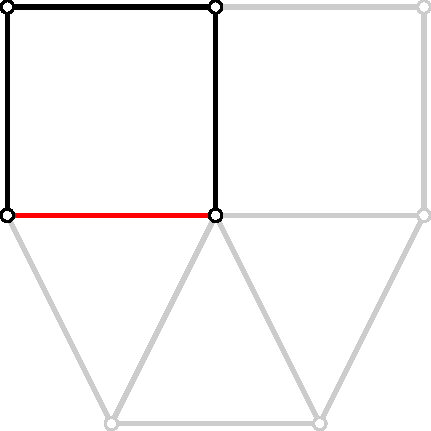
\includegraphics[width=0.17\hsize]{images/kirchhoff-10}&
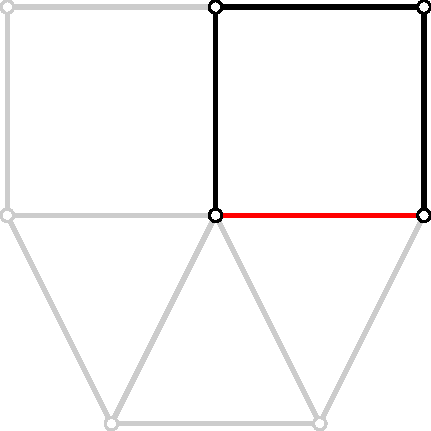
\includegraphics[width=0.17\hsize]{images/kirchhoff-6}&
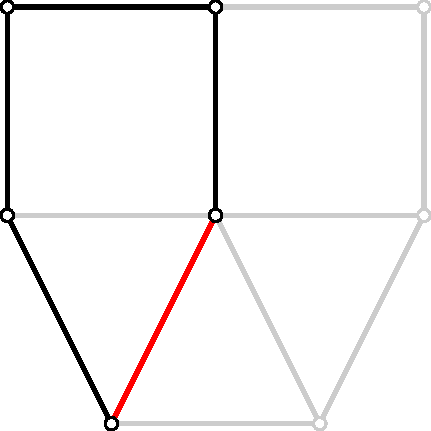
\includegraphics[width=0.17\hsize]{images/kirchhoff-7}&
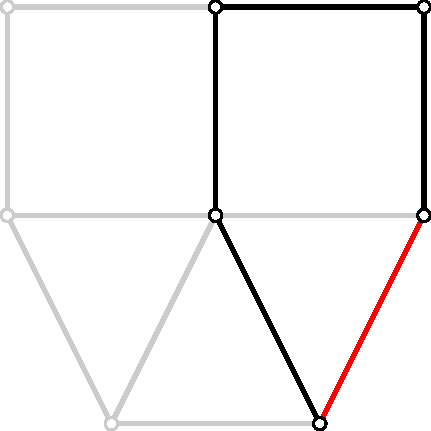
\includegraphics[width=0.17\hsize]{images/kirchhoff-8}&
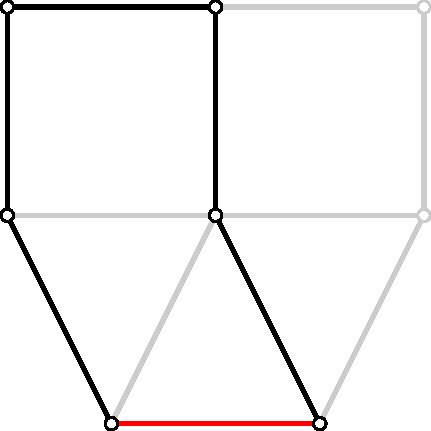
\includegraphics[width=0.17\hsize]{images/kirchhoff-9}\\
$z_1$&
$z_2$&
$z_3$&
$z_4$&
$z_5$\\
\end{tabular}
\end{center}
\caption{Basiszyklen des Netzwerkes aus
Abbildung~\ref{netzwerk-numeriert},
die frei w"ahlbaren Kanten jeweils rot hervorgehoben
\label{basiszyklen}}
\end{figure}
\begin{figure}
\begin{center}
\begin{tabular}{ccc}
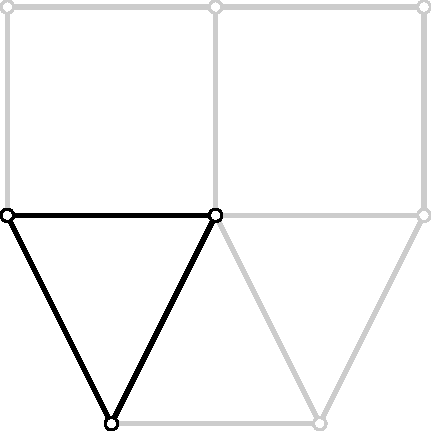
\includegraphics[width=0.17\hsize]{images/kirchhoff-11}&
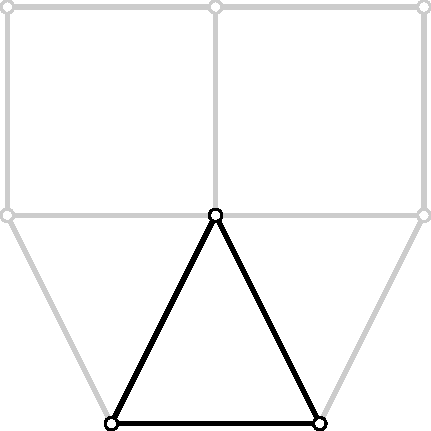
\includegraphics[width=0.17\hsize]{images/kirchhoff-12}&
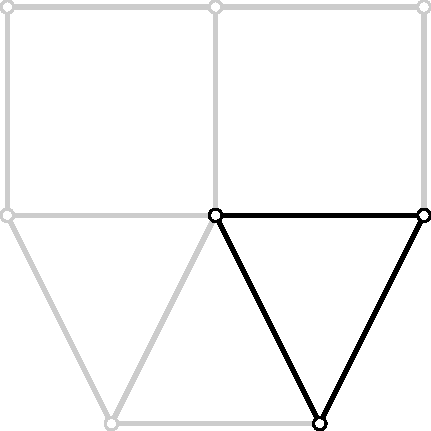
\includegraphics[width=0.17\hsize]{images/kirchhoff-13}\\
$-z_1+z_3$&
$-z_3+z_5$&
$-z_1+z_4$
\end{tabular}
\end{center}
\caption{Kombination der Dreiecke aus den Basiszyklen\label{dreiecke}}
\end{figure}
\index{Basiszyklen}

\subsubsection{Maschengleichungen}
Zu jedem Basiszyklus k"onnen wir jetzt gem"ass des ersten
Kirchhoffschen Gesetzes eine Gleichung bilden.
Seien $z_1,\dots,z_s$ die Basiszyklen.
Auf der linken Seite der Gleichungen muss jeder unbekannte Strom
auch noch mit dem Widerstand multipliziert werden.
Wir schreiben wir daf"ur die Diagonalmatrix
mit den Widerst"anden
\[
R=
\operatorname{diag}(R_1,R_2,\dots,R_n)=
\begin{pmatrix}
R_1&0&\dots&0\\
0&R_2&\dots&0\\
\vdots&\vdots&\ddots&\vdots\\
0&0&\dots&R_n
\end{pmatrix}
\]
und
$I$ f"ur den Spaltenvektor der gesuchten Str"ome. Dann ist $RI$
der Spaltenvektor mit den Produkten $R_iI_i$.
Schreiben wir ausserdem $e$ f"ur den
Spaltenvektor der elektromotorischen Kr"afte, dann 
werden die gesuchten Gleichungen
\begin{align*}
z_1^tRI&=z_1^te\\
&\;\vdots\\
z_s^tRI&=z_s^te.
\end{align*}
Schreiben wir die Zyklen als Spalten in eine Matrix $Z$, also f"ur das
Beispiel
\[
Z^t=
\begin{pmatrix}
1&0&-1&1&0&-1&0&0&0&0&0&0\\
0&1&0&-1&1&0&-1&0&0&0&0&0\\
-1&0&1&-1&0&0&0&1&-1&0&0&0\\
0&-1&0&1&-1&0&0&0&0&1&-1&0\\
1&0&-1&1&0&0&0&-1&0&1&0&-1
\end{pmatrix},
\]
dann werden die Gleichungen nach dem ersten Kirchhoffschen Gesetz
\[
Z^tRI=Z^te.
\]
Die gew"ahlte Konstruktion stellt automatisch sicher, dass die
Gleichungen linear unabh"angig sind, ja sie ermittelt sogar
die maximale Anzahl linear unabh"angiger Gleichungen.

\subsubsection{Der Rang von $\partial$}
Im Beispiel haben wir ein Netzwerk mit $n=12$ Knoten und $m=8$
Kanten untersucht, und darin $n-m+1=5$ Zyklen gefunden. Die Anzahl
der Zyklen l"asst sich aus dem Rang von $\partial$ ermitteln,
sie ist $n-\operatorname{Rang}\partial$. Um die Anzahl der
Basiszyklen zu bestimen, m"ussen wir also den Rang von $\partial$
bestimmen.

Jede Spalte von $\partial$ enth"alt genau eine $1$ und eine $-1$, also
verschwindet die Summe aller Zeilen von $\partial$.
Die Zeilen von $\partial$ sind also linear abh"angig, und es
gilt $\operatorname{Rang}\partial < m$. Wir k"onnen aber mehr
beweisen:

\begin{satz} $\operatorname{Rang}\partial = m-1$.
\label{partialrank}
\end{satz}

\begin{proof}[Beweis]
Wir f"uhren den Beweis mit vollst"andiger Induktion nach der Anzahl $n$
der Kanten des Netzwerks.
Dazu bauen wir das Netzwerk dadurch auf, dass wir nacheinander neue 
Kanten hinzuf"ugen, die an mindestens einem Ende mit einem Knoten
verbunden werden, der bereits mit mindestens einer Kante verbunden
ist. Wir m"ussen "uberpr"ufen, dass dabei der Rang von $\partial$
immer $m-1$ bleibt.

Induktionsverankerung: F"ur ein Netzwerk mit nur $m=2$ Knoten und
einer einzigen Kante ($n=1$) hat
$\partial$ die Form
\[
\partial=\begin{pmatrix}-1\\1\end{pmatrix},
\]
und hat offenbar Rang $1=m-1$. 

Nehmen wir jetzt an (Induktionsannahme), dass f"ur jedes Netzwerk mit $n-1$
Kanten die zugeh"orige $\partial$-Matrix den Rang $m-1$ hat,
wobei $m$ die Zahl der Knoten ist.
F"ugt man einen neue Kante hinzu, dann wird die Kantenzahl neu $n$.
Die Knotenzahl kann dabei gleich bleiben, oder auf $m+1$ anwachsen.

Im ersten Fall, als bei gleichbleibender Knotenzahl $m$,
weiss man nach Induktionsannahme, dass $m-1$ Zeilen
von $\partial$ immer linear unabh"angig sind.
Die zus"atzliche Spalte macht es noch schwieriger, eine lineare
Abh"angigkeit zu finden, der Rang von $\partial$ ist in diesem
Fall also $m-1$.

Im zweiten Fall wird die Matrix $\partial'$ des Netzwerkes mit
$n-1$ Kanten um eine Spalte (f"ur die neue Kante) und eine
Zeile (f"ur den zus"atzlichen Knoten) erweitert:
\[
\partial=
\left(
\begin{tabular}{>{$}c<{$}|>{$}c<{$}>{$}c<{$}>{$}c<{$}}
1& &0 & \\
\hline
& & & \\
-1& &\partial'& \\
&& &\\
\end{tabular}
\right)
\]
Der Gauss-Algorithmus entfernt im ersten Schritt die $-1$ in
der ersten Spalte, ohne dabei $\partial'$ zu ver"andern.
\[
\begin{tabular}{|>{$}c<{$}|>{$}c<{$}>{$}c<{$}>{$}c<{$}|}
\hline
1%
\begin{picture}(0,0)
\color{red}\put(-3,4){\circle{12}}
\end{picture}%
& &0 & \\
\hline
& & & \\
-1& &\partial'& \\
\begin{picture}(0,0)
\color{blue}\drawline(-10,-2)(-10,36)(10,36)(10,-2)
\end{picture}%
&& &\\
\hline
\end{tabular}
\rightarrow
\begin{tabular}{|>{$}c<{$}|>{$}c<{$}>{$}c<{$}>{$}c<{$}|}
\hline
1& &0 & \\
\hline
& & & \\
0& &\partial'& \\
&& &\\
\hline
\end{tabular}
\]
In den weiteren Schritten des Gauss-Algorithmus wird nur noch
die Matrix $\partial'$ ver"andert.
Insbesondere wird genau eine Null-Zeile entstehen, $\partial'$
hat nach Induktionsannahme den Rang $m-1$. Also hat $\partial$
den Rang $m$.
\end{proof}

\begin{satz}
Wenn durch Entfernung von $s=n-m+1$ Kanten $i_1,\dots,i_s$
eines Netzwerkes mit $n$ Ecken und $m$ Kanten alle Zyklen zerst"ort werden,
dann geh"ort jede der Kanten zu mindestens einem Zyklus.
\end{satz}

\begin{proof}[Beweis]
Es reicht zu zeigen, dass die erste Kante zu einem Zyklus geh"oren
muss. Entfernt man die Kante $i_1$, nimmt die Spaltenzahl von $\partial$
um $1$ ab, aber die Zeilen von $\partial$ bleiben linear abh"angig.
Die maximal m"ogliche Zahl linear unabh"angiger Zyklen muss also
ebenfalls um $1$ auf $s-1=n-m$ abnehmen.
Wenn andererseits $i_1$ in keinem Zyklus vorkommt, dann
bleiben die vorhandenen $s$ linear unabh"angigen Zyklen linear unabh"angig,
da die Zyklen an der Stelle $i_1$ alle die Komponenten $0$ haben.
Dieser Widerspruch zeigt, dass $i_1$ mindestens in einem Zyklus vorkommen
muss.
\end{proof}

\subsubsection{Das zweite Gesetz: die Knotenregel}
\index{Knotenregel}
\index{2. Kirchhoffsches Gesetz|see{Knotenregel}}
Das zweite Gesetz wird so formuliert:
\bigskip
\begin{center}
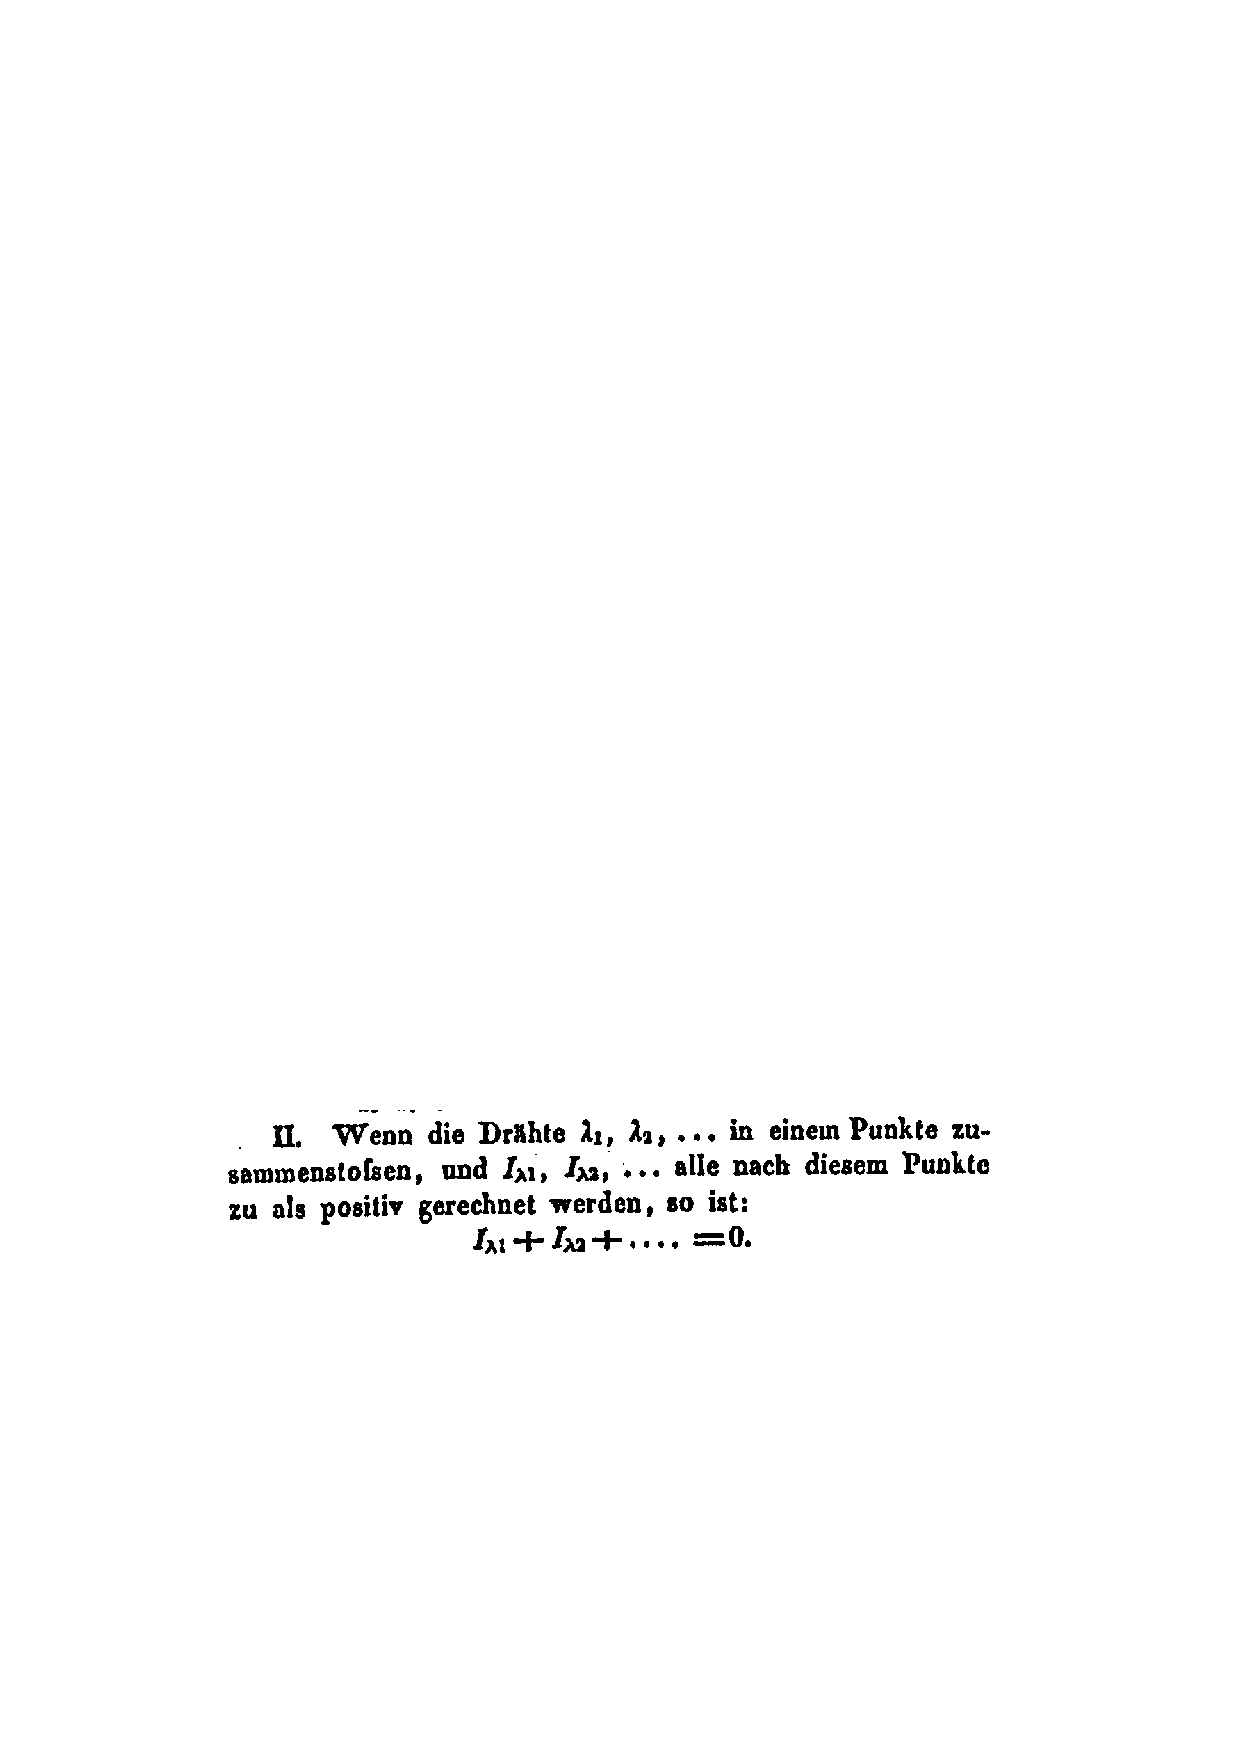
\includegraphics[width=\hsize]{graphics/kh2}
\end{center}
\bigskip
Im letzten Abschnitt haben wir jeder Kante eine Richtung gegeben,
wir rechnen den Strom positiv, wenn er in die gleiche Richtung fliesst
wie die Kante orientiert ist. F"ur die zweite Kirchhoffsche Regeln
m"ussen wir die $I_\lambda$ also noch mit den Gewichten der Kante
multiplizieren. Die Gewichte findet man in den Zeilen der Matrix
$\partial$, die Gleichungen nach der zweiten Kirchhoffschen
Regel sind also
\[
\partial I=0.
\]

In unserem Beispiel hatten wir f"unf Gleichungen aus der Maschenregel
f"ur die zw"olf unbekannten Str"ome ermittelt, die Knoten steuern
nochmals acht Gleichungen bei, so dass wir mit dreizehn Gleichungen
eine zu viel haben. Die Gleichungen m"ussen linear abh"angig sein,
aber welche der Gleichungen soll man weglassen?
Nach Satz~\ref{partialrank} ist $\operatorname{Rang}\partial=m-1$,
somit kann man jede beliebige der Gleichungen $\partial I=0$ weglassen.

Da also die Stromverteilung ein Zyklus sein muss, muss $I=Zj$ sein, wobei
$j$ ein Spaltenvektor ist, der die Str"ome "uber die frei w"ahlbaren
Kanten angibt. F"ur diese Str"ome folgen die Gleichungen
\[
Z^tRZj=Z^te,
\]
wir haben damit das Problem auf ein Gleichungssystem mit $n-m+1$
Gleichungen f"ur ebensoviele Unbekannten reduziert.
Die Koeffizientenmatrix $Z^tRZ$ des Gleichungssystems ist symmetrisch.

\subsubsection{Potential}
\index{Potential}
Um die Str"ome in einem Netzwerk zu messen, muss man die einzelnen
Dr"ahte auftrennen und ein Messger"at einf"ugen.
Spannungen zwischen zwei Knoten, also Potentialunterschiede,
sind viel einfacher zu messen.
Wir nehmen daher an, dass es einen $m$-dimensionalen
Potential-Vektor $U$ gibt.
Die Potentialdifferenz entlang einer Kante ist die Differenz
zwischen den Potentialen an den beiden Enden.
Da wir im $\partial$-Operator den Enden jeder Kante die Gewichte
$1$ und $-1$ gegeben haben, finden wir die n"otigen Koeffizienten
zur Berechnung der Potentialdifferenz in den Spalten von $\partial$.
Wir m"ussen also die Spalten von $\partial$ mit dem Spaltenvektor $U$
multiplizieren, diese sind aber die Zeilen von $\partial^t$.
Der Vektor der Potentialdifferenzen ist daher $\partial^t U$.

\index{Ohmsches Gesetz}
Das Ohmsche Gesetz besagt, dass die Str"ome proportional sind zu
den Potentialdifferenzen, also $\partial^t U=RI$, oder, wenn
wir f"ur die Matrix der Leitf"ahigkeiten $S=R^{-1}$ schreiben,
$I=S\partial^t U$. Die Maschengleichungen werden damit zu
\[
Z^t\partial^t U=Z^te
\]
Nun ist aber $Z^t\partial^t=(\partial Z)^t=0$, da $Z$ ja lauter
Zyklen als Spalten hat. Das Potential kann also genau dann verwendet
werden, wenn die elektromotorischen Kr"afte ich "uber jeden Zyklus zu $0$
summieren, und die
Maschengleichungen sind in diesem Fall automatisch erf"ullt.
Die Knotengleichungen werden zu
\[
\partial S\partial^tU=0.
\]
\index{Laplace-Operator}
Die Matrix $\Delta = \partial S\partial ^t$ heisst Laplace-Operator des
Netzwerks, offenbar ist $\Delta$ symmetrisch:
$\Delta^t=(\partial S\partial^t)^t
         =(\partial^t)^tS^t\partial^t
         =\partial S\partial^t
         =\Delta$.

Man kann $\Delta$ sehr leicht aus dem Netzwerk ablesen. Wir schreiben
$s_i=1/R_i$, also $S=\operatorname{diag}(s_1,\dots,s_m)$.
F"ur den Spezialfall
$R_i=1$ f"ur alle $i$ findet man zum Beispiel f"ur das Netzwerk
aus Abbildung~\ref{netzwerk-numeriert}:
\begin{equation}
\Delta
=
\partial \partial^t
=
\begin{pmatrix}
   2& -1&   & -1&   &   &   &   \\
  -1&  3& -1&   & -1&   &   &   \\
    & -1&  2&   &   & -1&   &   \\
  -1&   &   &  3& -1&   & -1&   \\
    & -1&   & -1&  5& -1& -1& -1\\
    &   & -1&   & -1&  3&   & -1\\
    &   &   & -1& -1&   &  3& -1\\
    &   &   &   & -1& -1& -1&  3
\end{pmatrix}
\label{samplelaplace}
\end{equation}
Fehlende Eintr"age sind als 0 zu lesen. Offenbar steht auf der Diagonalen
von $\Delta$ immer die Anzahl der Kanten, die in diesem 
Knoten zusammentreffen. F"ur beliebiges $S$ werden die Diagonalelemente
als Summe der Leitgf"ahigkeiten der in diesem Knoten zusammentreffenden
Kanten bestimmt.

Die Summe der Zeilen verschwindet, also ist $\Delta$ singul"ar.
Dies ist nicht weiter verwunderlich, denn das Potential ist ja nur
bis auf eine additive Konstante bestimmt. Man kann zu $U$ einen
konstanten Vektor hinzuaddieren, und erh"alt wieder eine L"osung.
Ein konstanter Vektor ist also eine L"osung des homogenen 
Gleichungssystems $\Delta U=0$
Man kann sich auch "uberzeugen, dass $\operatorname{Rang}\Delta = m-1$,
man muss also nur ein Potential w"ahlen (eine frei w"ahlbare Unbekannte),
um allen anderen Potentiale festzulegen.

\subsubsection{Externe Str"ome}
Das zweite Kirchhoffsche Gesetz geht davon aus, dass an den
Knoten keine externen Str"ome eingespeist oder abgezweigt werden.
Gilt diese Voraussetzung nicht mehr, wird die Knotengleichung zu
\begin{equation}
\partial I=I_{\text{ext}}
\qquad
\text{bzw.}
\qquad
\Delta U=I_{\text{ext}}.
\label{externestroeme}
\end{equation}

\subsubsection{Erweiterungen}
In der Elektrizit"atslehre lernt man, wie diese Theorie auf kontinuierliche
Stromverteilungen in einem leitenden Medium verallgemeinert werden kann,
dessen ortsabh"angige Leitf"ahigkeit $\sigma(x)$ bekannt ist.
Nennt man $\vec\jmath(x)$ den ortsabh"angigen
Vektor der Stromdichte, und $u(x)$ das Potential, dann gilt
$\vec\jmath(x)=\sigma(x)\operatorname{grad}(x)$, also
\[
\vec\jmath(x)=\sigma(x)\begin{pmatrix}
\frac{\partial u}{\partial x_1}\\
\frac{\partial u}{\partial x_2}\\
\frac{\partial u}{\partial x_3}
\end{pmatrix}.
\]
Die externen Str\"ome sind dann durch eine externe Stromdichte
$\vec\jmath_{\text{ext}}(x)$ gegeben, und es gilt
$\operatorname{div}\vec\jmath(x)=\vec\jmath_{\text{ext}}(x)$. Zusammen ergibt
sich die Gleichung
\[
\Delta_{\sigma}u(x)=\operatorname{div}\sigma(x)\operatorname{grad} u(x)=\vec\jmath_{\text{ext}}(x).
\]
Der Laplace-Operator $\Delta_\sigma$ ist also
\begin{align*}
\Delta_\sigma u(x)&=
\frac{\partial}{\partial x_1}\sigma(x)\frac{\partial u(x)}{\partial x_1}
+
\frac{\partial}{\partial x_2}\sigma(x)\frac{\partial u(x)}{\partial x_2}
+
\frac{\partial}{\partial x_3}\sigma(x)\frac{\partial u(x)}{\partial x_3}
\\
&=
\frac{\partial\sigma}{\partial x_1}\frac{\partial u}{\partial x_1}
+\sigma(x)\frac{\partial^2 u}{\partial x_1^2}+
\frac{\partial\sigma}{\partial x_2}\frac{\partial u}{\partial x_2}
+\sigma(x)\frac{\partial^2 u}{\partial x_2^2}+
\frac{\partial\sigma}{\partial x_3}\frac{\partial u}{\partial x_3}
+\sigma(x)\frac{\partial^2 u}{\partial x_3^2}.
\end{align*}
Es ist also eine lineare partielle Differentialgleichung zu l"osen.

